\documentclass{standalone}

\usepackage{amsmath,amssymb}

\usepackage{tikz}
\usetikzlibrary{quantikz}
\usetikzlibrary{decorations.pathmorphing}
\usetikzlibrary{shapes.arrows}
\usetikzlibrary{calc,math}

\usetikzlibrary{quantikz}
\usepackage{physics}

\newcommand{\on}[1]{\operatorname{#1}}


\begin{document}

\tikzset{every picture/.style={line width=0.75pt}} %set default line width to 0.75pt        

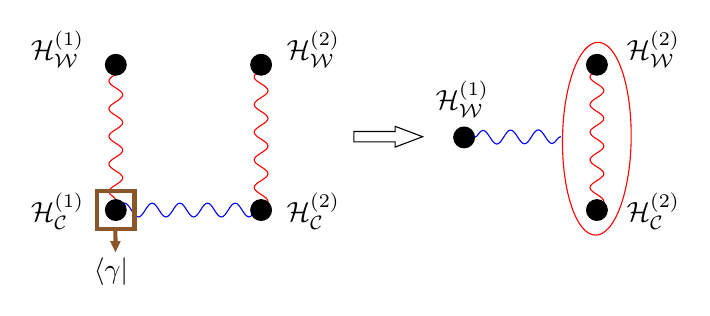
\begin{tikzpicture}[x=0.75pt,y=0.75pt,yscale=-1,xscale=1]
%uncomment if require: \path (0,300); %set diagram left start at 0, and has height of 300
%Straight Lines [id:da21088942034957192] 
\draw  [draw=red, decorate, decoration=snake]  (45,62) -- (45,135) ;
%Straight Lines [id:da5410877290710232] 
\draw  [draw=red, decorate, decoration=snake]  (115,60) -- (115,135) ;
%Straight Lines [id:da730027415704626] 
\draw  [draw=blue, decorate, decoration=snake]  (45,135) -- (115,135) ;
%Shape: Circle [id:dp9854151274628302] 
\draw  [fill={rgb, 255:red, 0; green, 0; blue, 0 }  ,fill opacity=1 ] (40,65) .. controls (40,62.24) and (42.24,60) .. (45,60) .. controls (47.76,60) and (50,62.24) .. (50,65) .. controls (50,67.76) and (47.76,70) .. (45,70) .. controls (42.24,70) and (40,67.76) .. (40,65) -- cycle ;
%Shape: Circle [id:dp8966133290287497] 
\draw  [fill={rgb, 255:red, 0; green, 0; blue, 0 }  ,fill opacity=1 ] (40,135) .. controls (40,132.24) and (42.24,130) .. (45,130) .. controls (47.76,130) and (50,132.24) .. (50,135) .. controls (50,137.76) and (47.76,140) .. (45,140) .. controls (42.24,140) and (40,137.76) .. (40,135) -- cycle ;
%Shape: Circle [id:dp5805720403493042] 
\draw  [fill={rgb, 255:red, 0; green, 0; blue, 0 }  ,fill opacity=1 ] (110,65) .. controls (110,62.24) and (112.24,60) .. (115,60) .. controls (117.76,60) and (120,62.24) .. (120,65) .. controls (120,67.76) and (117.76,70) .. (115,70) .. controls (112.24,70) and (110,67.76) .. (110,65) -- cycle ;
%Shape: Circle [id:dp767403568793527] 
\draw  [fill={rgb, 255:red, 0; green, 0; blue, 0 }  ,fill opacity=1 ] (110,135) .. controls (110,132.24) and (112.24,130) .. (115,130) .. controls (117.76,130) and (120,132.24) .. (120,135) .. controls (120,137.76) and (117.76,140) .. (115,140) .. controls (112.24,140) and (110,137.76) .. (110,135) -- cycle ;
%Right Arrow [id:dp0988377616542766] 
\draw   (159.67,97.17) -- (179.57,97.17) -- (179.57,94.67) -- (192.83,99.67) -- (179.57,104.67) -- (179.57,102.17) -- (159.67,102.17) -- cycle ;
%Shape: Rectangle [id:dp24725342060756206] 
\draw  [color={rgb, 255:red, 139; green, 87; blue, 42 }  ,draw opacity=1 ][line width=1.5]  (36,126) -- (54,126) -- (54,144) -- (36,144) -- cycle ;
%Straight Lines [id:da7435547473684463] 
\draw [color={rgb, 255:red, 139; green, 87; blue, 42 }  ,draw opacity=1 ][line width=1.5] (44.8,143.8) -- (44.82,152.33) ;
\draw [shift={(44.83,155.33)}, rotate = 269.83] [fill={rgb, 255:red, 139; green, 87; blue, 42 }  ,fill opacity=1 ][line width=0.08]  [draw opacity=0] (5.36,-2.57) -- (0,0) -- (5.36,2.57) -- cycle    ;
%Straight Lines [id:da6038206266107193] 
\draw [draw=blue, decorate, decoration=snake] (259.4,99.6) -- (212.8,100) ;
%Straight Lines [id:da6980552336067618] 
\draw  [draw=red, decorate, decoration=snake]  (276.8,60) -- (276.8,135) ;
%Shape: Circle [id:dp7674121181277671] 
\draw  [fill={rgb, 255:red, 0; green, 0; blue, 0 }  ,fill opacity=1 ] (207.8,100) .. controls (207.8,97.24) and (210.04,95) .. (212.8,95) .. controls (215.56,95) and (217.8,97.24) .. (217.8,100) .. controls (217.8,102.76) and (215.56,105) .. (212.8,105) .. controls (210.04,105) and (207.8,102.76) .. (207.8,100) -- cycle ;
%Shape: Circle [id:dp5465628832571865] 
\draw  [fill={rgb, 255:red, 0; green, 0; blue, 0 }  ,fill opacity=1 ] (271.8,65) .. controls (271.8,62.24) and (274.04,60) .. (276.8,60) .. controls (279.56,60) and (281.8,62.24) .. (281.8,65) .. controls (281.8,67.76) and (279.56,70) .. (276.8,70) .. controls (274.04,70) and (271.8,67.76) .. (271.8,65) -- cycle ;
%Shape: Circle [id:dp5577767638934235] 
\draw  [fill={rgb, 255:red, 0; green, 0; blue, 0 }  ,fill opacity=1 ] (271.8,135) .. controls (271.8,132.24) and (274.04,130) .. (276.8,130) .. controls (279.56,130) and (281.8,132.24) .. (281.8,135) .. controls (281.8,137.76) and (279.56,140) .. (276.8,140) .. controls (274.04,140) and (271.8,137.76) .. (271.8,135) -- cycle ;
%Shape: Ellipse [id:dp15923894457168264] 
\draw [draw=red]  (260.22,100.41) .. controls (260.58,74.76) and (268.29,54.07) .. (277.42,54.2) .. controls (286.55,54.33) and (293.66,75.23) .. (293.29,100.88) .. controls (292.93,126.53) and (285.22,147.22) .. (276.09,147.09) .. controls (266.96,146.96) and (259.85,126.06) .. (260.22,100.41) -- cycle ;

% Text Node
\draw (2.8,47.4) node [anchor=north west][inner sep=0.75pt]    {$\mathcal{H}^{( 1)}_{\mathcal{W}}$};
% Text Node
\draw (126,47.4) node [anchor=north west][inner sep=0.75pt]    {$\mathcal{H}^{( 2)}_{\mathcal{W}}$};
% Text Node
\draw (2.8,125.4) node [anchor=north west][inner sep=0.75pt]    {$\mathcal{H}^{( 1)}_{\mathcal{C}}$};
% Text Node
\draw (126,125.4) node [anchor=north west][inner sep=0.75pt]    {$\mathcal{H}^{( 2)}_{\mathcal{C}}$};
% Text Node
\draw (33.13,156.73) node [anchor=north west][inner sep=0.75pt]    {$\langle \gamma |$};
% Text Node
\draw (197.8,71.4) node [anchor=north west][inner sep=0.75pt]    {$\mathcal{H}^{( 1)}_{\mathcal{W}}$};
% Text Node
\draw (289.8,47.4) node [anchor=north west][inner sep=0.75pt]    {$\mathcal{H}^{( 2)}_{\mathcal{W}}$};
% Text Node
\draw (289.8,125.4) node [anchor=north west][inner sep=0.75pt]    {$\mathcal{H}^{( 2)}_{\mathcal{C}}$};
\end{tikzpicture}

\end{document}
